\documentclass{article}

% Packages
\usepackage{geometry}
\usepackage{graphicx}
\usepackage{lipsum}
\usepackage{listings}
\usepackage{float}
\usepackage[portuguese]{babel}
\DeclareUnicodeCharacter{2212}{\ensuremath{-}}

% Page setup
\geometry{a4paper, margin = 2 cm}

\begin{document}

% cover
\thispagestyle{empty} % Remove page number from first page

\begin{figure}[t]
    
\includegraphics[width=3cm]{images/logo-puc-minas.png}
    \hspace{0.02\textwidth}
    \vline%
    \hspace{0.04\textwidth}
    
\includegraphics[width=3cm]{images/logo-icei.jpeg}
\end{figure}

\hrulefill%
\vspace{\baselineskip}

\Large\noindent
\textbf{Pontifícia Universidade Católica de Minas Gerais} \\
\textbf{Instituto de Ciências Exatas e Informática} \\
\textbf{Departamento de Engenharia de Computação}

\begin{center}
    \vfill
    \Huge\textbf{Relatório: Trabalho Prático 2} \\
    \vspace{0.5 cm}
    \Large\textbf{NP Completo - Partição} \\
    \vspace{1 cm}
    \large \textbf{Professor}: Walisson Ferreira de Carvalho \\
    \vspace{0.5 cm}
    \large Arthur Gonçalves Ayres Lanna  \\
    \large Marcus Leandro Gomes Campos Oliveira \\
    \large Rafael Ramos de Andrade \\
    \vfill
    \large Belo Horizonte \\ Campus Coração Eucarístico \\
    \vspace{\baselineskip}
    \large \today
\end{center}

% table of contents
\newpage
\thispagestyle{empty}
\tableofcontents

% body
\newpage
\large % document text size

\section{Introdução}

Os problemas NP-completos ocupam um lugar de destaque na ciência da computação devido à sua complexidade intrínseca e relevância prática. Esses problemas pertencem à classe \emph{NP} (nondeterministic polynomial time), que engloba aqueles cuja solução pode ser verificada em tempo polinomial. Para que um problema seja classificado como NP-completo, ele deve satisfazer duas condições fundamentais: ser pertencente à classe \emph{NP} e ser pelo menos tão difícil quanto qualquer outro problema em \emph{NP}, no sentido de que qualquer problema em \emph{NP} pode ser reduzido a ele por meio de uma transformação em tempo polinomial. Essa propriedade foi formalizada por Stephen Cook em 1971, no famoso \emph{Teorema de Cook}, que estabeleceu o primeiro problema NP-completo, o problema da satisfatibilidade booleana (\emph{SAT}).

O problema da Partição, foco deste trabalho, é um exemplo clássico de problema NP-completo. Ele consiste em determinar se um conjunto finito de números inteiros pode ser dividido em dois subconjuntos cuja soma dos elementos seja igual. Formalmente, dado um vetor \( S \) de números inteiros, o objetivo é encontrar dois subconjuntos disjuntos \( S_1 \) e \( S_2 \), tais que \( S_1 \cup S_2 = S \) e \( \sum_{x \in S_1} x = \sum_{x \in S_2} x \). O problema é diretamente relacionado ao \emph{Subset Sum Problem} e, consequentemente, ao problema da mochila (\emph{Knapsack Problem}), ambos também pertencentes à categoria NP-completo.

Historicamente, o problema da Partição foi amplamente estudado devido à sua simplicidade na formulação e à complexidade subjacente na solução. Embora o conceito seja mencionado em literatura matemática desde o século XIX, sua formalização no contexto de algoritmos e complexidade computacional ganhou relevância durante a segunda metade do século XX, impulsionada pelo avanço da teoria da computação e pelo interesse em resolver problemas combinatórios desafiadores.

As aplicações do problema da Partição são variadas e abrangem diversas áreas práticas. Na computação, ele é frequentemente utilizado em algoritmos de balanceamento de carga, onde tarefas devem ser distribuídas de maneira equitativa entre dois ou mais processadores. Na otimização de sistemas, o problema aparece em cenários como alocação de recursos e particionamento de redes. Além disso, possui implicações em teoria de jogos e análise de riscos financeiros, onde é necessário balancear custos ou benefícios entre diferentes participantes.

Apesar de sua dificuldade computacional, o problema da Partição é de grande relevância prática, motivando o desenvolvimento de algoritmos eficientes, tanto exatos quanto heurísticos, para lidar com instâncias específicas. Este trabalho busca explorar as características do problema, analisar algoritmos clássicos e propor implementações que contribuam para o entendimento de sua solução e impacto prático.

\section{Algoritmos}

\item \textbf{Recursão simples}: A abordagem recursiva explora todas as possíveis partições do conjunto, caracterizando-se por uma complexidade exponencial \(O(2^n)\). Apesar de ser conceitualmente simples, essa abordagem não é eficiente, dado o número significativo de subproblemas repetidos, o que a torna impraticável para conjuntos maiores~\cite{cormen2009introduction}.

\item \textbf{Top-Down com memoization}: Essa técnica melhora a eficiência da recursão utilizando uma tabela (ou cache) para armazenar os resultados dos subproblemas já resolvidos. Dessa forma, evita-se a recalculação redundante, reduzindo a complexidade para \(O(n \cdot T)\), onde \(T\) é a soma total dos elementos do conjunto. O uso de memoization é especialmente vantajoso em problemas onde apenas uma parte das combinações possíveis é explorada, como no cálculo de subsequências ou caminhos otimizados~\cite{cormen2009introduction}.

\item \textbf{Bottom-Up com tabulação}: Neste método, resolve-se os subproblemas menores iterativamente, partindo dos casos base até o problema completo. A tabulação utiliza uma tabela para armazenar os resultados intermediários de forma sistemática, garantindo que cada subproblema seja resolvido uma única vez. Essa abordagem elimina a sobrecarga de chamadas recursivas e o risco de estouro de pilha, com a mesma eficiência de \(O(n \cdot T)\). Exemplos incluem algoritmos para subsequências e cálculo de somas parciais~\cite{cormen2009introduction, garey1979computers}.

\item \textbf{Bottom-Up com otimização de espaço}: Esta variação da tabulação reduz o consumo de memória ao utilizar apenas o armazenamento necessário para resolver o subproblema atual. Em vez de manter uma tabela completa, utiliza-se um número fixo de variáveis ou uma estrutura compacta que armazena apenas as últimas iterações relevantes. Essa técnica é eficiente em problemas lineares, como a resolução do problema da mochila ou subsequências~\cite{cormen2009introduction, garey1979computers}.
\end{itemize}

\section{Versão NP Difícil}

A versão NP-hard do problema da partição surge em contextos onde os elementos do conjunto possuem pesos adicionais ou restrições complexas, como no problema da partição com pesos (\textit{Weighted Partition Problem}) ou com múltiplos subconjuntos. Nessa variante, o objetivo é dividir o conjunto $S = \{s_1, s_2, \dots, s_n\}$ em $k$ subconjuntos disjuntos \( S_1, S_2, \dots, S_k \), tal que as somas dos pesos em cada subconjunto estejam equilibradas, enquanto se respeitam restrições adicionais, como dependências entre os elementos.

Ao contrário da versão clássica, esta generalização é NP-hard, pois aumenta significativamente o espaço de soluções possíveis e incorpora características de outros problemas difíceis, como o problema do caixeiro-viajante (\textit{Traveling Salesman Problem}) e o problema de particionamento de grafos (\textit{Graph Partitioning})~\cite{garey1979computers, papadimitriou1994computational}. 

Essa variante é amplamente utilizada em otimização de sistemas distribuídos, onde o balanceamento de carga entre servidores deve considerar não apenas o volume de trabalho, mas também a conectividade e a latência entre os componentes~\cite{martello1981knapsack}.

\section{Metodologia}

\section{Resultados e análise}
Os testes foram realizados em uma máquina com Ryzen 7 5700x e 33 GB de RAM 3200 MHz e os gráficos gerados utilizando Pandas e MatPlotLib.

\subsection{Tempo de execução}

Ao analisarmos os tempos de execução, é possível observar a diferença significativa entre as implementações usando programação dinâmica e heurística em relação ao uso da força bruta (reta amarela). Para vetores maiores que 22 a implementação por força bruta domina assintoticamente todas as outras implementações. No entanto, para tamanhos menores que 22, ela se mostra extremamente rápida, executando 7 vezes mais rápida que a implementação utilizando programação dinâmica bottom-up.

\begin{figure} [H]
    \centering
    \caption{Tempo de execução x Tamanho do vetor}
    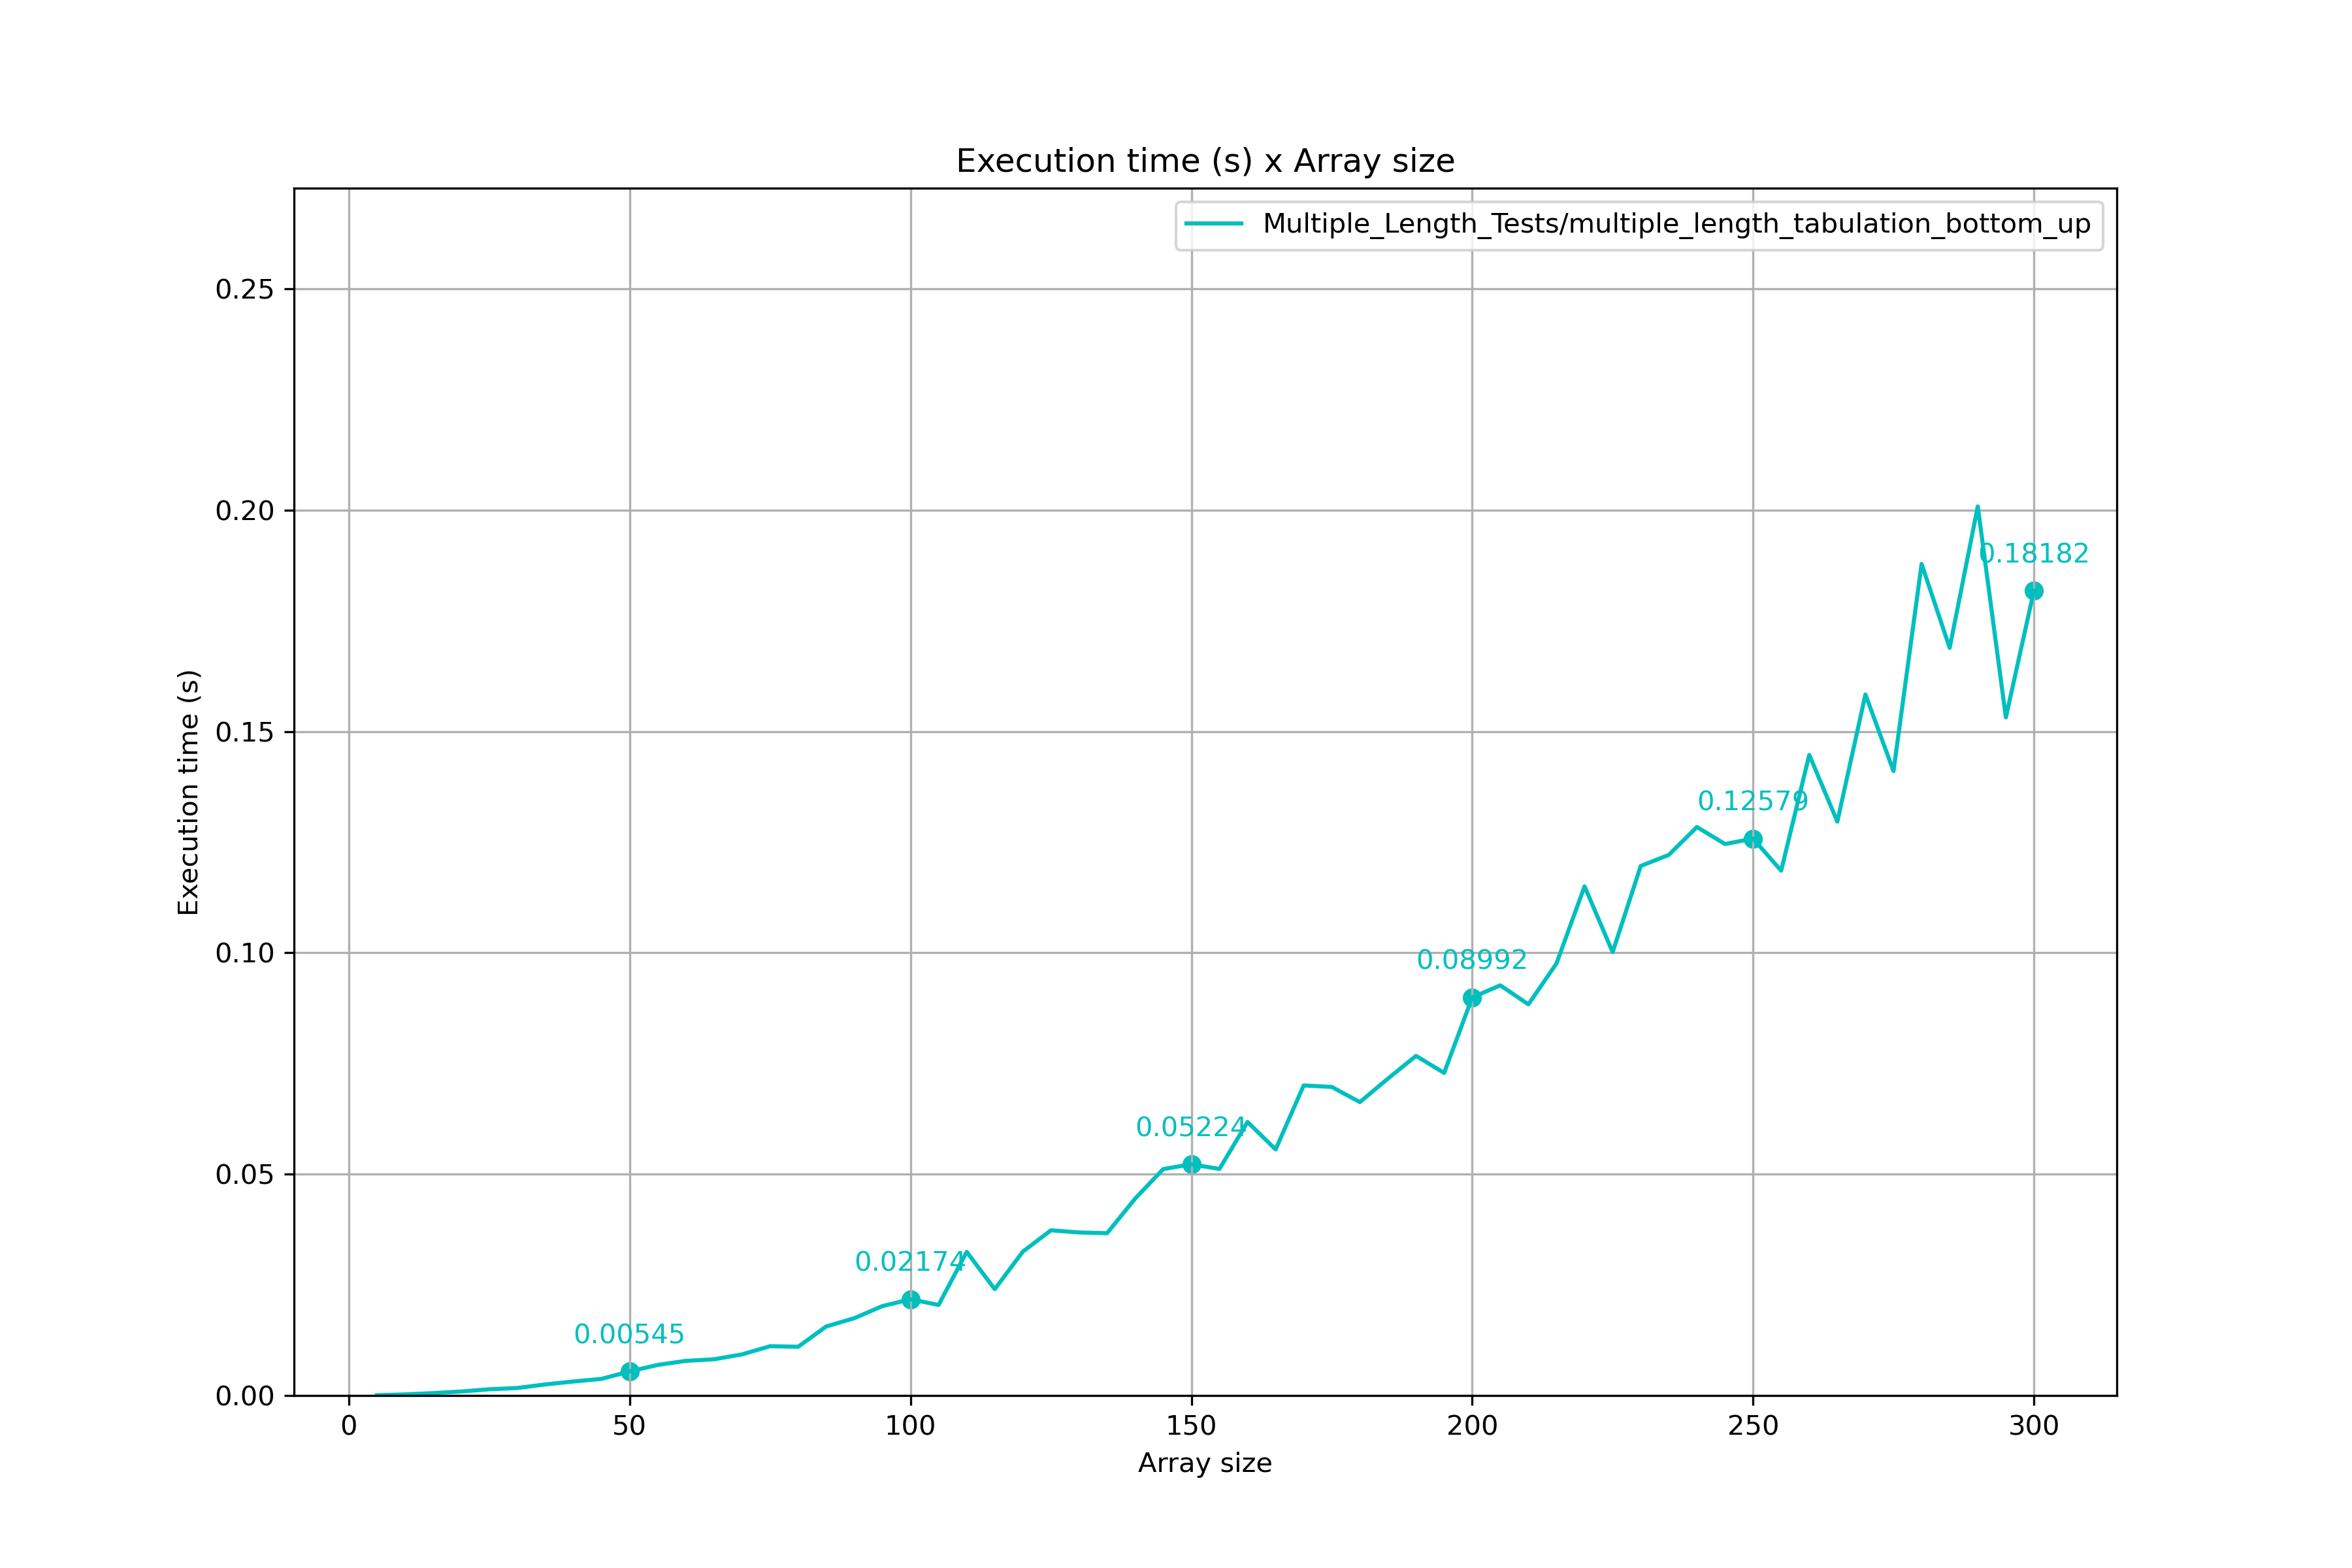
\includegraphics[width=1\textwidth]{images/multiple_length_tabulation_bottom_up}
\end{figure}

\subsection{Comparação entre heurística}


\section{Conclusão}


\bibliographystyle{plain}
\bibliography{references}
\begin{thebibliography}{99}
\bibitem{garey1979computers} Garey, M. R., \& Johnson, D. S. (1979). \textit{Computers and Intractability: A Guide to the Theory of NP-Completeness}. W. H. Freeman.
\bibitem{karp1972reducibility} Karp, R. M. (1972). Reducibility Among Combinatorial Problems. \textit{Complexity of Computer Computations}, 85-103.
\bibitem{martello1981knapsack} Martello, S., \& Toth, P. (1981). \textit{Knapsack Problems: Algorithms and Computer Implementations}. Wiley.
\bibitem{cormen2009introduction} Cormen, T. H., Leiserson, C. E., Rivest, R. L., \& Stein, C. (2009). \textit{Introduction to Algorithms} (3rd ed.). MIT Press.
\bibitem{papadimitriou1994computational} Papadimitriou, C. H. (1994). \textit{Computational Complexity}. Addison-Wesley.
\end{thebibliography}

\section{Anexo}

\end{document}
